\section*{Signalanalyse}
\label{sec:Signalanalyse}
\subsection*{Anschlagserkennung}
Zur Erkennung von von Anschlägen und Abgrenzung von Hintergrundrauschen werden die Messdaten in Echtzeit geprüft. Hierzu werden die jeweils letzten beiden Messwerte miteinander verglichen. Ein Anschlag wird erkannt, wenn der aktuellere Wert den vorherigen Wert um ein bestimmtes Vielfaches der Standartabweichung übersteigt. Der Faktor sollte dabei auf das zu erwartende Rauschen abgestimmt werden - höhere Werte neigen weniger dazu, Ausschläge im Rauschen bzw. unabsichtliche Behrührungen der Oberfläsche als Anschlag zu erkennen, niedrigere Werte erlauben dagegen, auch sanfte Anschläge zu erkennen. In unseren Versuchen hat sich ein Faktor von 6 als stabil erwiesen.

Wurde ein Anschlag erkannt, so beginnt ein Zeitfenster von ca. 500ms, in dem eingehende Messwerte gepuffert werden. Nach Ablauf des Zeitfensters wird dem Programm signalisiert, dass ein Schlag aufgenommen wurde. Zusätzlich werden die Messwerte bis ca. 20ms vor dem erkannten Anschlag in die Zeitreihe aufgenommen.

\subsection*{Analyse der Beschleunigungsdaten}
Die Klassifizierung aufgenommener Schläge erfolgt mittels Auswertung der stärksten Frequenzen. Hierzu werden die Messwerte zunächst einer diskreten Fouriertransformation unterzogen, die Spektrale Leistungssdichte der Zeitreihe bestimmt.
In der aktuellen Implementierung konnten Abtastraten von ca. 200Hz erreicht werden. 
Für ein Zeitfenster von ca. 500ms ergeben sich somit 128 Messwerte. 
Nach Anwendung der Fouriertransformation erhält man somit 64 diskrete Frequenzgruppen mit einer Trennschärfe von ca. 2Hz.

Aus diesen Daten werden die 4 Frequenzanteile mit der höchsten Leistungsdichte ermittelt zur weiteren Verwendung gespeichert.

\subsection*{Lernphase}
Zum Erlernen einer Schlagposition werden 10 Schläge aufgezeichnet und der Durchschnitt der jeweils stärksten Frequenzgruppe, zweitstärksten Frequenzgruppe, usw... ermittelt. Diese werden als charakteristisches Pattern gespeichert.
Tabelle \ref{tab:FFT} zeigt die zwölf Schläge zum Lernen für Hihat und Bass.
Die Schläge wurden auf einer Tischplatte ausgeführt mit 

\begin{figure}[H]
	\centering
	\caption{Stärkste Frequenzen}
	\begin{tabular}{l c c c c | l c c c c}
		HiHat &&&& &Bass \\
		\hline
		Frequenz & F1 & F2 & F3 & F4  & & F1 & F2 & F3 & F4\\	
		& 13 & 14 & 15 & 19  &&13& 114& 115& 87\\
		& 30 & 31 & 23 & 24 &&13& 28& 29& 30\\
		& 13& 14& 15& 16 &&35& 36& 23& 24\\
		& 29& 30& 13&36 &&13& 14& 15& 62\\
		& 17& 23&24& 30 	&&15& 16& 42& 43\\
		&13& 24& 25& 47	&&13& 54& 30& 31\\

		&27& 15& 16& 17	&&20& 89& 90& 39\\

		 &17& 18& 30& 31 &&13& 20& 26& 27\\

		&42& 43& 44& 55		&&19& 20& 29& 30\\

		 &25& 33& 34& 35 &&19& 20& 13& 26 \\

		&22& 23& 13& 37		&&13& 14& 15& 16\\

		&31& 32& 14& 15  &&13& 58& 59& 60\\
		\\
		\hline
		Durchschnitt & 23,25&	25	&22,167& 30,167 && 16,583	&40,25&	40,5&	39,583	\\
		Median & 23,5 &	23,5& 19,5	& 30,5 && 13 &	24	& 29	 &30,5 \\		 
		

	\end{tabular}
	\label{tab:FFT}
\end{figure}

\begin{figure}[H]
\centering
\begin{subfigure}{.5\textwidth}
		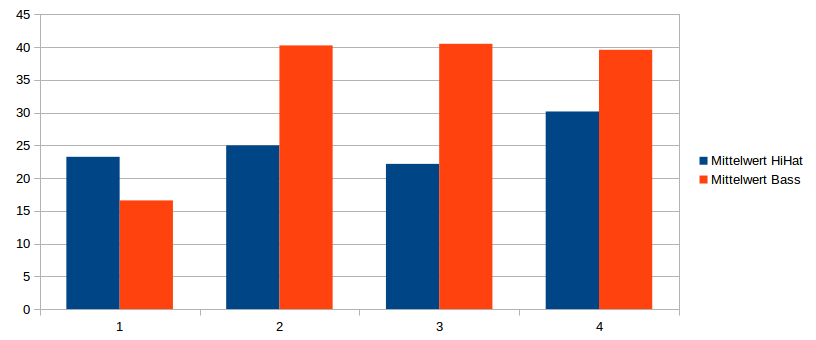
\includegraphics[scale=0.5]{figures/Mittelwert_hihatbass.png}
\end{subfigure}
\caption{Mittelwerte von Hihat und Bass für Frequenzen F1 - F4}
\label{fig:FFT_Mittelwerte}
\end{figure}


\begin{figure}[H]
\centering
\begin{subfigure}{.5\textwidth}
		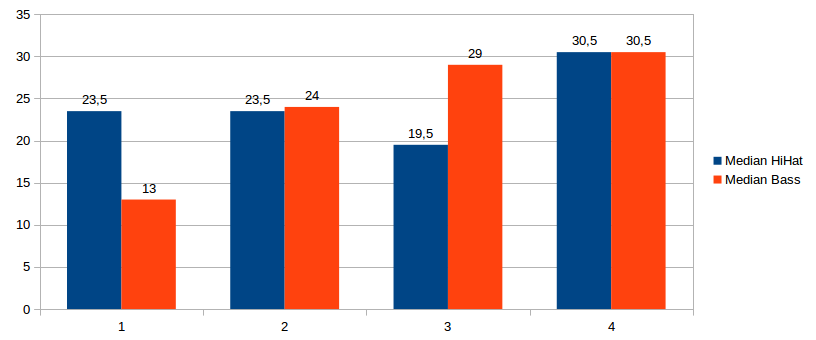
\includegraphics[scale=0.5]{figures/Median_hihatbass.png}
\end{subfigure}
\caption{Median-Werte  von Hihat und Bass für Frequenzen F1 - F4}
\label{fig:FFT}
\end{figure}


\subsection*{Echtzeit-Klassifizierung}
Ist die Echtzeit-Klassifizierung aktiviert, so werden nach erfolgter Anschlagserkennung und Schlagaufzeichnung die Messwerte analysiert und die stärksten Frequenzgruppen mit denen der gelernten Positionen verglichen. Der Schlag wird der Position mit der gerinsten totalen Abweichung zugeordnet.
Erkennbar hierbei ist, dass in jedem Falle eine Zuordnung erfolgt - auch wenn die Abweichung absurd groß ist. Dies könnte jedoch leicht geändert werden, indem eine maximale Abweichung festgelegt wird und alle berechneten Abweichungen, die diesen Wert übersteigen, als nicht klassifizierbar eingestuft werden. Alternativ könnte, ähnlich zu anderen Clustering-Verfahren, eine Nachbarschaftsbeziehung zur Klassifikation verwendet werden.

\subsection*{Signalaufbereitung/Filterung}

In der aktuellen Implementierung erfolgt keine Filterung oder Nachbereitung der Messwerte. 


Eine Möglichkeit, um Rauschen zu unterdrücken wäre die Nutzung eines Grenzwertes. Auf diese Art können schwache Erschütterungen und leichte Vibrationen unterdrückt werden.
Die Sensordaten könnten weiter geglättet werden durch Verwendung eines Box-Filters (Moving-Average) oder Gauss-Filters.

%Anstelle von timbreID, welches laut Entwickler \cite{timbreID} Cluster benutzt und Merkmale sortiert, haben wir den DBSCAN-Algorithmus getetest.

%Elbatta und Ashour untersuchen verschiedene Clustering Ansätze und stellen in ihrer Arbeit \cite{Elbatta2013ADM} einen verbesserten DBSCAN-Algorithmus vor.
%DBSCAN ist ein  dichtebasierter Cluster-Algorithmus, der als Parameter einen Radius und eine Mindestanzahl an Punkte pro Cluster benötigt.
%Im Gegensatz zu partitionierungsbasierten Cluster-Algorithmen, wie zum Beispiel K-Means, besitzt DBSCAN dne Vorteil, dass es freie Formen von Clustern erkennen kann und sich besonders gut für Daten mit %Rauschen eignet.
%Der Algorithmus startet mit einem zufälligen Punkt.
%Befinden sich die Mindestanzahl an Nachbarpunkten um den gewählten Punkt im gegebenen Radius, wird ein Cluster mit allen gefunden Punkten gebildet.
%Ist die Anzahl Nachbarpunkte kleiner als die Mindestanzahl wird dies als Rauschen markiert.
%Es wird rekursiv mit dem nächsten freien Punkt verfahren, der noch nicht zu einem Cluster gehört und noch nicht bewertet wurde.

%Der DBSCAN-Algorithmus könnte somit verwendet werden, um besondere Merkmale von festzustellen und diese von Rauschen zu unterscheiden.

%Ein Clustering mit DBSCAN zeigte bei uns keine guten Ergebnisse, da wohl die Merkmale
